\documentclass[size=a4, parskip=half, titlepage=false, toc=flat, toc=bib, 12pt]{scrartcl}

\setuptoc{toc}{leveldown}

% Ajuste de las líneas y párrafos
\linespread{1.2}
\setlength{\parindent}{0pt}
\setlength{\parskip}{12pt}

% Español
\usepackage[spanish, es-tabla]{babel}

% Matemáticas
\usepackage{amsmath}
\usepackage{amsthm}

% Links
%\usepackage{hyperref}

% Fuentes
\usepackage{newpxtext,newpxmath}
\usepackage[scale=.9]{FiraMono}
\usepackage{FiraSans}
\usepackage[T1]{fontenc}

\defaultfontfeatures{Ligatures=TeX,Numbers=Lining}
\usepackage[activate={true,nocompatibility},final,tracking=true,factor=1100,stretch=10,shrink=10]{microtype}
\SetTracking{encoding={*}, shape=sc}{0}

\usepackage{graphicx}
\usepackage{float}

% Mejores tablas
\usepackage{booktabs}

\usepackage{adjustbox}

% COLORES

\usepackage{xcolor}

\definecolor{verde}{HTML}{007D51}
\definecolor{esmeralda}{HTML}{045D56}
\definecolor{salmon}{HTML}{FF6859}
\definecolor{amarillo}{HTML}{FFAC12}
\definecolor{morado}{HTML}{A932FF}
\definecolor{azul}{HTML}{0082FB}
\definecolor{error}{HTML}{b00020}

% ENTORNOS
\usepackage[skins, listings, theorems]{tcolorbox}

\newtcolorbox{recuerda}{
  enhanced,
%  sharp corners,
  frame hidden,
  colback=black!10,
	lefttitle=0pt,
  coltitle=black,
  fonttitle=\bfseries\sffamily\scshape,
  titlerule=0.8mm,
  titlerule style=black,
  title=\raisebox{-0.6ex}{\small RECUERDA}
}

\newtcolorbox{nota}{
  enhanced,
%  sharp corners,
  frame hidden,
  colback=black!10,
	lefttitle=0pt,
  coltitle=black,
  fonttitle=\bfseries\sffamily\scshape,
  titlerule=0.8mm,
  titlerule style=black,
  title=\raisebox{-0.6ex}{\small NOTA}
}

\newtcolorbox{error}{
  enhanced,
%  sharp corners,
  frame hidden,
  colback=error!10,
	lefttitle=0pt,
  coltitle=error,
  fonttitle=\bfseries\sffamily\scshape,
  titlerule=0.8mm,
  titlerule style=error,
  title=\raisebox{-0.6ex}{\small ERROR}
}

\newtcblisting{shell}{
  enhanced,
  colback=black!10,
  colupper=black,
  frame hidden,
  opacityback=0,
  coltitle=black,
  fonttitle=\bfseries\sffamily\scshape,
  %titlerule=0.8mm,
  %titlerule style=black,
  %title=Consola,
  listing only,
  listing options={
    style=tcblatex,
    language=sh,
    breaklines=true,
    postbreak=\mbox{\textcolor{black}{$\hookrightarrow$}\space},
    emph={jmml@UbuntuServer, jmml@CentOS},
    emphstyle={\bfseries},
  },
}

\newtcbtheorem[number within=section]{teor}{\small TEOREMA}{
  enhanced,
  sharp corners,
  frame hidden,
  colback=white,
  coltitle=black,
  fonttitle=\bfseries\sffamily,
  %separator sign=\raisebox{-0.65ex}{\Large\MI\symbol{58828}},
  description font=\itshape
}{teor}

\newtcbtheorem[number within=section]{prop}{\small PROPOSICIÓN}{
  enhanced,
  sharp corners,
  frame hidden,
  colback=white,
  coltitle=black,
  fonttitle=\bfseries\sffamily,
  %separator sign=\raisebox{-0.65ex}{\Large\MI\symbol{58828}},
  description font=\itshape
}{prop}

\newtcbtheorem[number within=section]{cor}{\small COROLARIO}{
  enhanced,
  sharp corners,
  frame hidden,
  colback=white,
  coltitle=black,
  fonttitle=\bfseries\sffamily,
  %separator sign=\raisebox{-0.65ex}{\Large\MI\symbol{58828}},
  description font=\itshape
}{cor}

\newtcbtheorem[number within=section]{defi}{\small DEFINICIÓN}{
  enhanced,
  sharp corners,
  frame hidden,
  colback=white,
  coltitle=black,
  fonttitle=\bfseries\sffamily,
  %separator sign=\raisebox{-0.65ex}{\Large\MI\symbol{58828}},
  description font=\itshape
}{defi}

\newtcbtheorem{ejer}{\small EJERCICIO}{
  enhanced,
  sharp corners,
  frame hidden,
  left=0mm,
  right=0mm,
  colback=white,
  coltitle=black,
  fonttitle=\bfseries\sffamily,
  %separator sign=\raisebox{-0.65ex}{\Large\MI\symbol{58828}},
  description font=\itshape,
  nameref/.style={},
}{ejer}

% CÓDIGO
\usepackage{listings}

% CABECERAS
\pagestyle{headings}
\setkomafont{pageheadfoot}{\normalfont\normalcolor\sffamily\small}
\setkomafont{pagenumber}{\normalfont\sffamily}

% ALGORITMOS
\usepackage[vlined,linesnumbered]{algorithm2e}
\usepackage{listings}
\usepackage{color}
\renewcommand{\lstlistingname}{Listado}

\definecolor{dkgreen}{rgb}{0,0.6,0}
\definecolor{gray}{rgb}{0.5,0.5,0.5}
\definecolor{mauve}{rgb}{0.58,0,0.82}

\lstset{frame=tb,
  language=Python,
  aboveskip=3mm,
  belowskip=3mm,
  showstringspaces=false,
  columns=flexible,
  basicstyle={\small\ttfamily},
  numbers=none,
  numberstyle=\tiny\color{gray},
  keywordstyle=\color{blue},
  commentstyle=\color{dkgreen},
  stringstyle=\color{mauve},
  breaklines=true,
  breakatwhitespace=true,
  tabsize=2
}

% Formato de los pies de figura
\setkomafont{captionlabel}{\scshape}
\SetAlCapFnt{\normalfont\scshape}
\SetAlgorithmName{Algoritmo}{Algoritmo}{Lista de algoritmos}

% BIBLIOGRAFÍA
%\usepackage[sorting=none]{biblatex}
%\addbibresource{bibliografia.bib}

\begin{document}

\renewcommand{\proofname}{\normalfont\sffamily\bfseries\small DEMOSTRACIÓN}

\title{Trabajo 2\\
Programación}
\subject{Aprendizaje automático}
\author{Johanna Capote Robayna\\
    5 del Doble Grado en Informática y Matemáticas\\
    Grupo A}
\date{}
\publishers{\vspace{2cm}
\includegraphics[height=2.5cm]{UGR}\vspace{1cm}}
\maketitle

\newpage

\tableofcontents
\newpage

\section{Ejercicio sobre la complejidad de H y el ruido}
Este ejercicio se desarrolla en el archivo \verb|ejercicio1.py|.

\begin{enumerate}
\item Dibujar una gráfica con la nube de puntos de salida correspondiente.
\begin{enumerate}
\item Considere $N = 50$, $dim = 2$, $rango = [−50, +50]$ con \verb|simula_unif(N, dim, rango)|.
\begin{figure}[H]
\centering
\spanishdecimal{.}
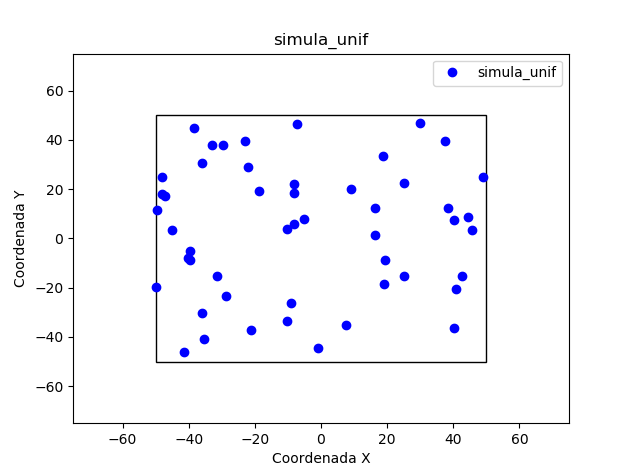
\includegraphics[width=0.7\textwidth]{./img/unif}
\caption{Nube de puntos generados uniformemente en $[-50,50]x[-50,50]$.}
\end{figure}
Para comprobar que efectivamente los puntos se encuentran dentro de las regiones se ha dibujado un rectángulo cuya esquina inferior izquierda es $[-50, -50]$ y con longitud de altura y anchura $100$. Podemos comprobar que todos los puntos se encuentran dentro del rectángulo y que se distribuyen de manera uniforme.
\item Considere $N = 50$, $dim = 2$ y $sigma = [5, 7]$ con \verb|simula_gaus(N, dim, sigma)|.
\begin{figure}[H]
\centering
\spanishdecimal{.}
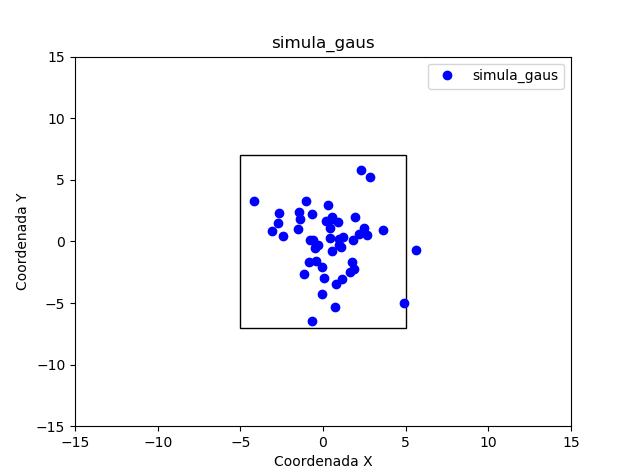
\includegraphics[width=0.7\textwidth]{./img/gauss}
\caption{Nube de puntos generada a partir de una Gaussiana de media $0$ y varianzas $5$ y $7$.}
\end{figure}

Por otro lado en este caso también se se ha dibujado un rectángulo cuya esquina inferior izquierda es $[-5, -7]$ y con longitud de altura $10$ y anchura $14$. En este caso la función no obliga a que lo puntos se encuentren dentro de los margenes, por lo que pueden haber puntos fuera pero pegados a la frontera como ocurre en este caso, por otro lado vemos como los puntos tienden a juntarse en el centro.
\end{enumerate}

\item Vamos a valorar la influencia del rudio en la seleccion de la complejidad de la clase de
funciones. Con ayuda de la función \verb|simula_unif(100, 2, [−50, 50])| generar una muestra
de puntos 2D a los que vamos añadir una etiqueta usando el signo de la función $f(x, y) =
y − ax − b$, es decir el signo de la distancia de cada punto a la recta simulada con
\verb|simula_recta()|.

\begin{enumerate}
\item Dibujar una gráfica donde los puntos muestren el resultado de su etiqueta,
junto con la recta usada para ello.
\begin{figure}[H]
\centering
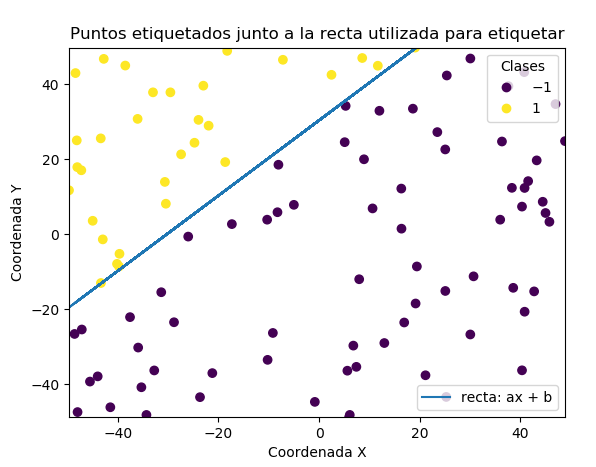
\includegraphics[width=0.7\textwidth]{./img/sinruido}
\caption{Nube de puntos etiquetados sin ruido.}
\end{figure}
\item Modifique de forma aleatoria un 10 % etiquetas positivas y otro 10 %
de negativas y guarde los puntos con sus nuevas etiquetas. Dibuje de nuevo la gráfica
anterior.
\begin{figure}[H]
\centering
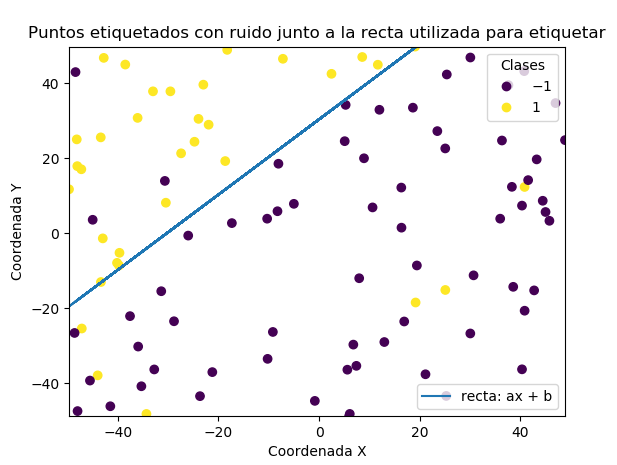
\includegraphics[width=0.7\textwidth]{./img/conruido}
\caption{Nube de puntos etiquetados con ruido.}
\end{figure}
\item Supongamos ahora que las siguientes funciones definen la frontera de
clasificación de los puntos de la muestra en lugar de una recta.
\begin{itemize}
\item $f(x, y) = (x − 10)^2 + (y − 20)^2 − 400$
\item $f(x, y) = 0,5(x + 10)^2 + (y − 20)^2 − 400$
\item $f(x, y) = 0,5(x − 10)^2 − (y + 20)^2 − 400$
\item $f(x, y) = y − 20x^2 − 5x + 3$
\end{itemize}

Visualizar el etiquetado generado en 2b junto con cada una de las gráficas de cada una
de las funciones. Comparar las regiones positivas y negativas de estas nuevas funciones
con las obtenidas en el caso de la recta. ?`Son estas funciones más complejas mejores
clasificadores que la función lineal? Observe las gráficas y diga que consecuencias
extrae sobre la influencia del proceso de modificación de etiquetas en el proceso de
aprendizaje. Explicar el razonamiento.
\begin{figure}[H]
\centering
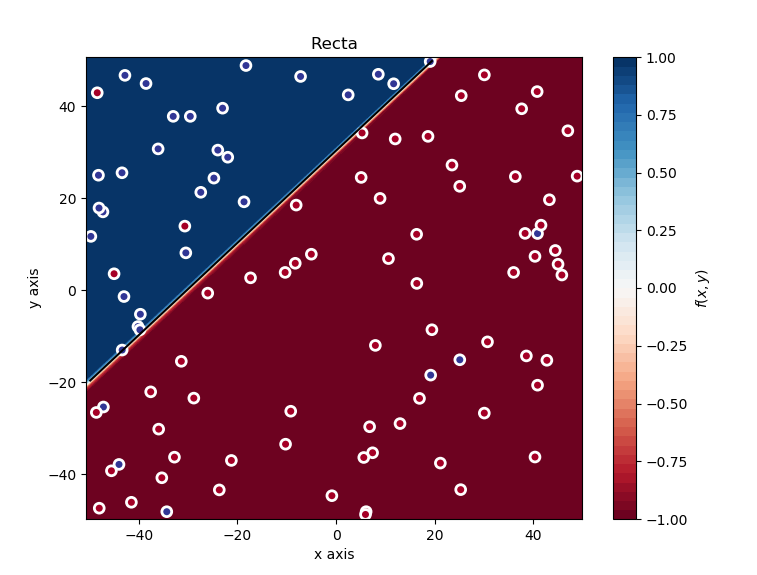
\includegraphics[width=0.7\textwidth]{./img/recta}
\caption{Recta $f(x,y) = y - ax - b$.}
\end{figure}
\begin{figure}[H]
\centering
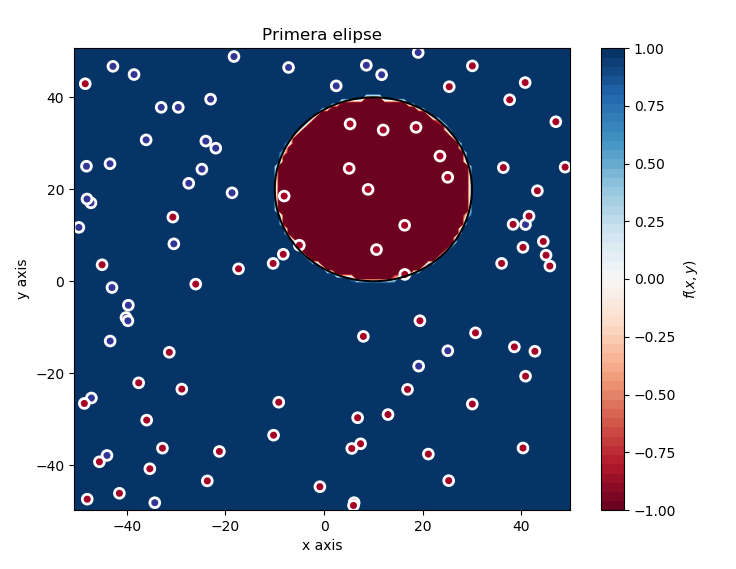
\includegraphics[width=0.7\textwidth]{./img/elipse1}
\caption{Elipse 1 $f(x, y) = (x − 10)^2 + (y − 20)^2 − 400$.}
\end{figure}
\begin{figure}[H]
\centering
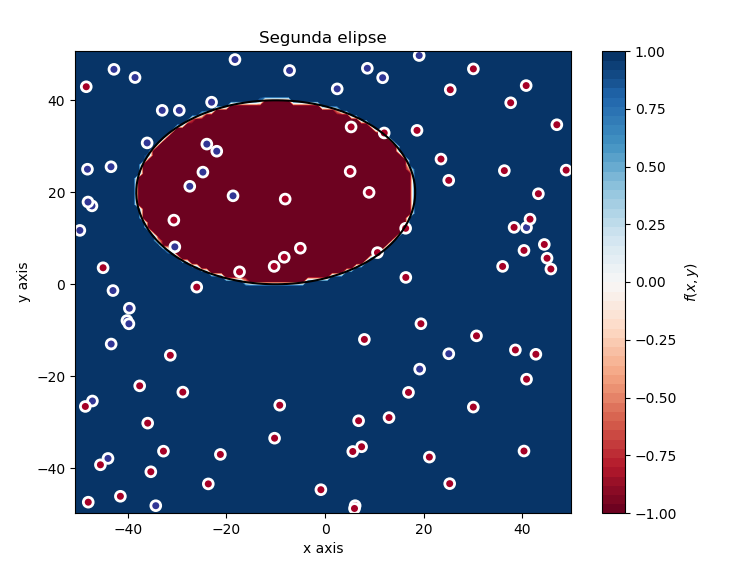
\includegraphics[width=0.7\textwidth]{./img/elipse2}
\caption{Elipse 2 $f(x, y) = 0,5(x + 10)^2 + (y − 20)^2 − 400$.}
\end{figure}
\begin{figure}[H]
\centering
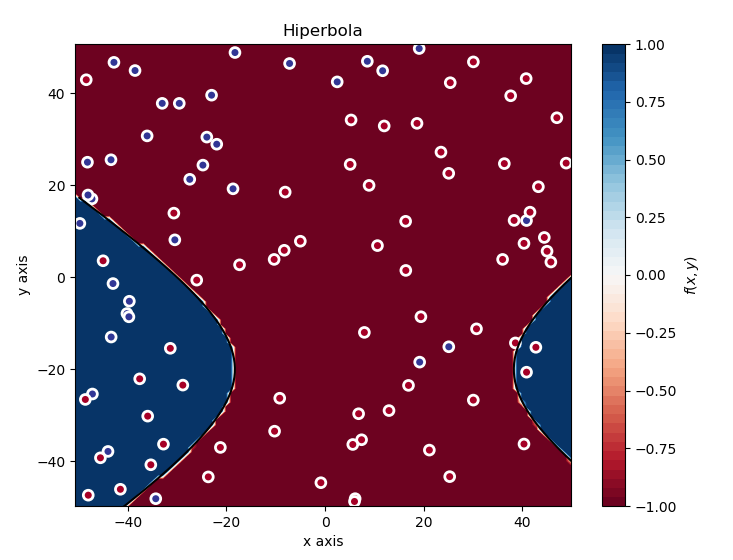
\includegraphics[width=0.7\textwidth]{./img/hiperbola}
\caption{Hipérbola $f(x, y) = 0,5(x − 10)^2 − (y + 20)^2 − 400$.}
\end{figure}
\begin{figure}[H]
\centering
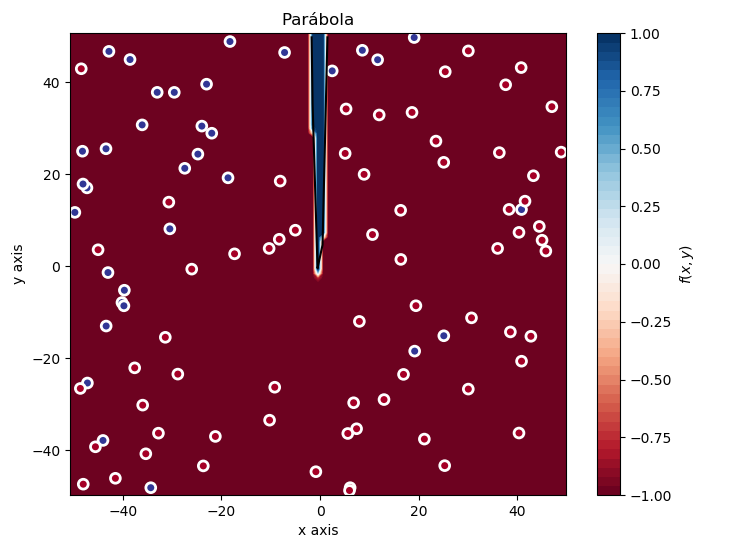
\includegraphics[width=0.7\textwidth]{./img/parabola}
\caption{Parábola $f(x, y) = y − 20x^2 − 5x + 3$.}
\end{figure}
Para evaluar la bondad de estos clasificadores se pide que utilicemos como métrica el porcentaje de puntos bien clasificados.
\begin{verbatim}
Porcentaje de aciertos de la recta:
91.0
Porcentaje de aciertos de la primera elipse:
46.0
Porcentaje de aciertos de la segunda elipse:
38.0
Porcentaje de aciertos de la hiperbola:
61.0
Porcentaje de aciertos de la parábola:
66.0
\end{verbatim}

Nos damos cuenta de que al aumentar la complejidad del clasificador no aumenta el porcentaje de aciertos, esto es debido a que hemos utilizado para etiquetar una recta y el porcentaje de ruido es bajo.

Por otro lado si nos fijamos en la parábola, esta clasifica la mayoría de puntos como ``rojos''y ha dado la casualidad de que en nuestro conjunto la mayoría de puntos son rojos, por lo que este clasificador obtiene un porcentaje de aciertos bastante alto. Esto último es un error, ya que consideraríamos la parábola con un clasificador decente cuando a simple vista se comprueba que no. El error reside en  que la métrica utilizada para establecer la bondad de los clasificadores no es la más oportuna.

\end{enumerate}
\end{enumerate}

\section{Modelos lineales}
Este ejercicio se ha implementado en el archivo \verb|ejercicio2.py|.
\subsection{Algoritmo Perceptron}
\begin{enumerate}
\item Ejecutar el algoritmo PLA con los datos simulados en los apartados 2a de la
sección.1. Inicializar el algoritmo con: a) el vector cero y, b) con vectores de
números aleatorios en $[0, 1]$ (10 veces). Anotar el número medio de iteraciones
necesarias en ambos para converger. Valorar el resultado relacionando el punto
de inicio con el número de iteraciones.

Como el algoritmo es determinista solo ejecutamos el experimento con el vector cero una vez, ya que para un mismo punto inicial el algoritmo obtiene el mismo resultado.

\spanishdecimal{.}
Vemos que en el caso del vector cero necesita $34$ épocas para converger mientras que empezando con distintos vectores aleatorios necesita de media $124.2$ iteraciones. Podemos observar que el punto de inicio no influye en el número de iteraciones necesarias para converger.
\begin{verbatim}
Vector 0
Iteraciones: 34
Porcentaje correctos: 100.0

Vetores aleatorios
Valor medio de iteraciones necesario para converger: 124.2
Valor medio del porcentaje de aciertos: 100.0
\end{verbatim}

En la siguiente gráfica vemos como el porcentaje de aciertos crece.
\begin{figure}[H]
\centering
\spanishdecimal{.}
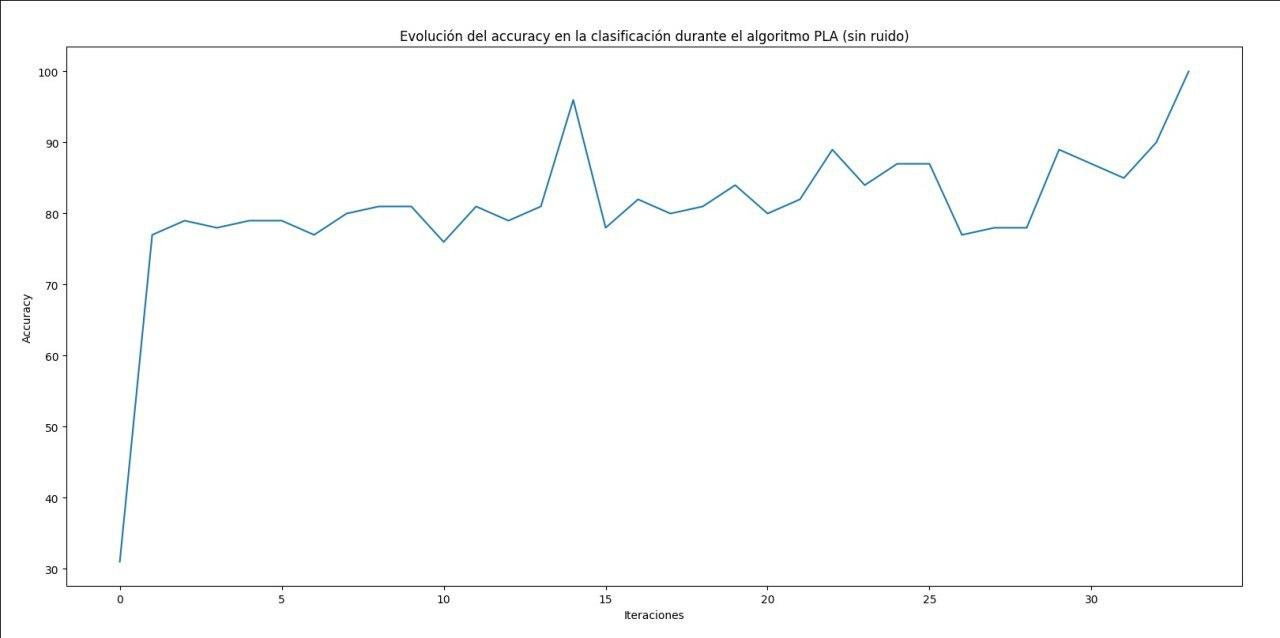
\includegraphics[width=0.7\textwidth]{./img/accsinruido}
\caption{Evolución de la tasa de aciertos.}
\end{figure}

Además observamos que al no haber ruido en el conjunto de datos la recta obtenida con el algoritmo consigue separar los datos con un porcentaje de aciertos del $100\%$.

\begin{figure}[H]
\centering
\spanishdecimal{.}
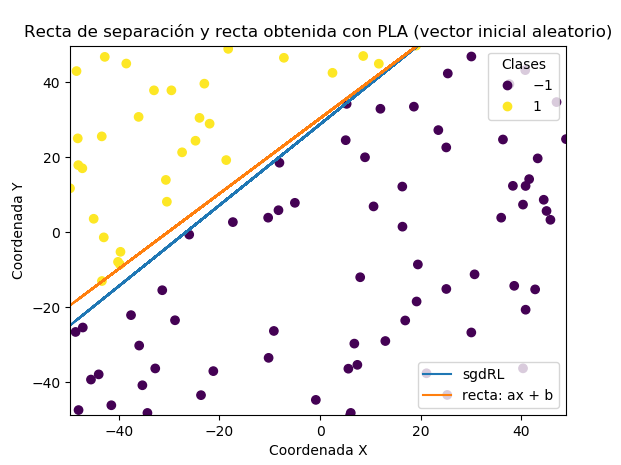
\includegraphics[width=0.7\textwidth]{./img/2a1}
\caption{Recta separadora junto con recta obtenida con PLA.}
\end{figure}

\item Hacer lo mismo que antes usando ahora los datos del apartado 2b de la sección.1.
?`Observa algún comportamiento diferente? En caso afirmativo diga cual y las
razones para que ello ocurra.

Al igual que antes ejecutamos el algoritmo con el vector cero solo una vez ya que el algoritmo es determinista.

Observamos que en este caso al incorporar ruido en la muestra el algoritmo nunca llega a converger, es decir alcanza el número máximo de iteraciones ($1000$ épocas). Esto es lógico ya que es imposible llegar a separar correctamente todos los puntos mediante una recta.

\begin{verbatim}
Vector 0
Iteraciones: 1000
Procentaje correctos: 81.0


Vetores aleatorios
Valor medio de iteraciones necesario para converger: 1000.0
Valor medio del porcentaje de aciertos: 75.3
\end{verbatim}

En la siguiente gráfica vemos como el porcentaje de aciertos oscila.
\begin{figure}[H]
\centering
\spanishdecimal{.}
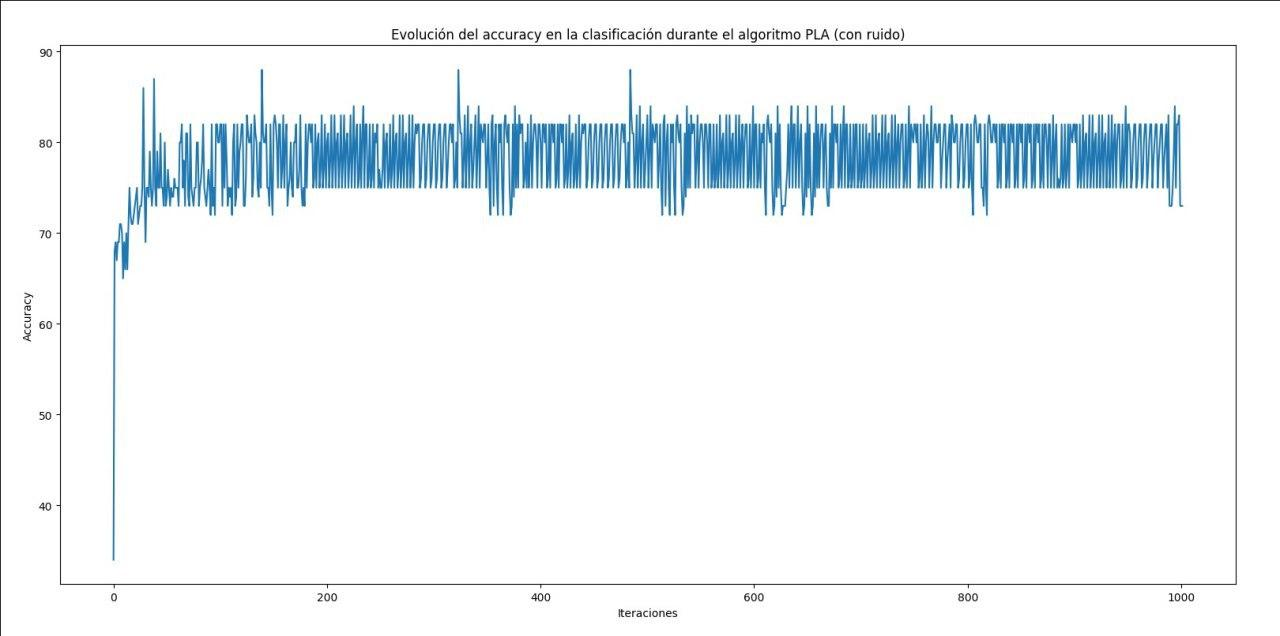
\includegraphics[width=0.7\textwidth]{./img/accconruido}
\caption{Evolución de la tasa de aciertos.}
\end{figure}
\end{enumerate}

Comprobamos gráficamente los resultados obtenidos:
\begin{figure}[H]
\centering
\spanishdecimal{.}
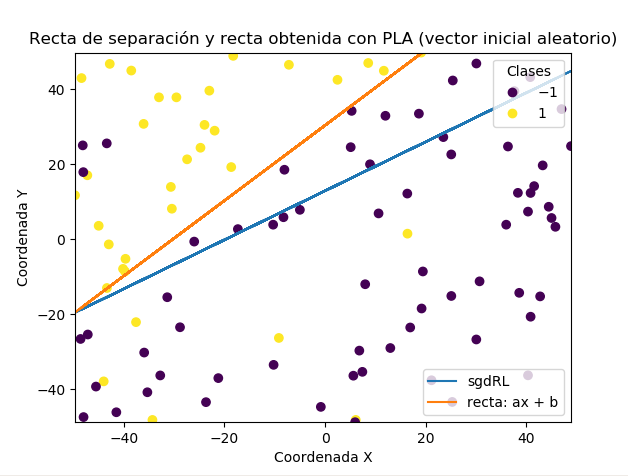
\includegraphics[width=0.7\textwidth]{./img/2a2}
\caption{Recta separadora junto con recta obtenida con PLA.}
\end{figure}

\subsection{Regresión logística}
\begin{enumerate}
\item Implementar Regresión Logística(RL) con Gradiente Descendente Estocástico
(SGD) bajo las siguientes condiciones:

Para implementar el algoritmo se han declarado dos funciones: \verb|sgdRL| donde se encuentra el código princpial, en el que buscamos minimizar el error logístico con SGD, y \verb|gradRL| donde se encuentra ya desarrollada la expresión del gradiente del error logistico:
$$E_{in}(w) = \frac{1}{N} \sum_{n=1}^N log(1 + e^{-y_n w^T x_n}) $$
$$\triangledown_w E_{in}(w) = \frac{-1}{N} \sum_{n=1}^N \frac{y_nx_n}{1 + e^{y_n w^Tx_n}}$$


\item Usar la muestra de datos etiquetada para encontrar nuestra solución g y estimar
$E_{out}$ usando para ello un número suficientemente grande de nuevas muestras
$(>999)$.

Con la muestra de datos etiquetadas utilizamos el algoritmo diseñado en el apartado anterior para obtener la función $g$. A continuación, generamos un conjunto \textit{test} de datos uniformemente distribuidos de tamaño $1000$, lo etiquetamos con la función del ejercicio 1 y calculamos el error logístico de $g$. Además añadimos el porcentaje de aciertos para comprobar la bondad del resultado.
\begin{verbatim}
Bondad del resultado para grad. descendente estocastico:

Eout:  0.11378017016196812
Porcentaje de aciertos 98.6
\end{verbatim}

Vemos que el error logistico es muy pequeño y que el porcentaje de puntos mal clasificados es solo un $1.4\%$.

\begin{figure}[H]
\centering
\spanishdecimal{.}
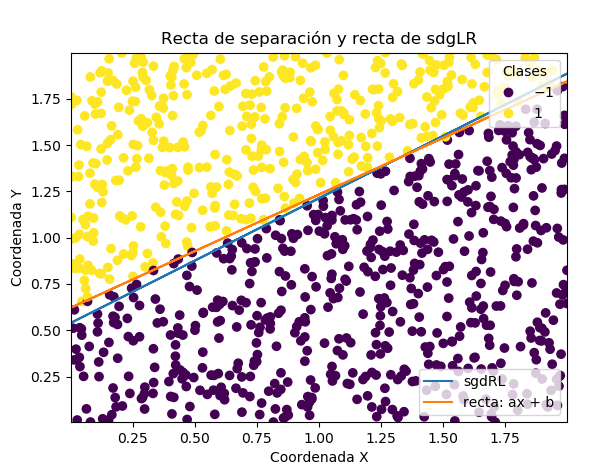
\includegraphics[width=0.7\textwidth]{./img/2b}
\caption{Conjunto de datos test junto con la recta separadora y la generada con sgdRL}
\end{figure}

\end{enumerate}

\section{BONUS}
Este apartado se ha desarrollados en el archivo \verb|bonus.py|.

\begin{enumerate}
\item Plantear un problema de clasificación binaria que considere el conjunto de entrenamiento como datos de entrada para aprender la función $g$.

Planteamos un problema de clasificación con los siguientes elementos:
\begin{itemize}
\item Espacio de entrada: $X = {1} x \mathbb{R}^2$
\item Espacio de etiquetas: $Y = \{-1, 1\}$
\item Espacio de funciones candidatas: $H = \{ f:X \rightarrow Y | \exists w \in \mathbb{R}^3 f(x) = w^T x \}$
\item Conjunto de muestra $D \subset X x Y$ muestra aleatoria simple de tamaño 1194 de la distribución desconocida $P(X,Y)$ tal que $f(x) = P(y|x)$ donde $f$ es la función que etiqueta.
\item Criterio de aprendizaje (ERM): $w^* = argmin_w \frac{1}{1194} \sum_{i=1}^{1194} loss_w(x_i,y_i)$
\item Función de pérdida: $loss_w(x,y) = [[w^Tx = y]]$
\end{itemize}

\item Usar un modelo de Regresión Lineal y aplicar PLA-Pocket como mejora. Responder
a las siguientes cuestiones.

Como algoritmo para obtener la regresión lineal hemos utilizado el de la pseudo-inversa.
\spanishdecimal{.}
\begin{enumerate}
\item Generar gráficos separados (en color) de los datos de entrenamiento y test junto
con la función estimada.

\begin{figure}[H]
\centering
\spanishdecimal{.}
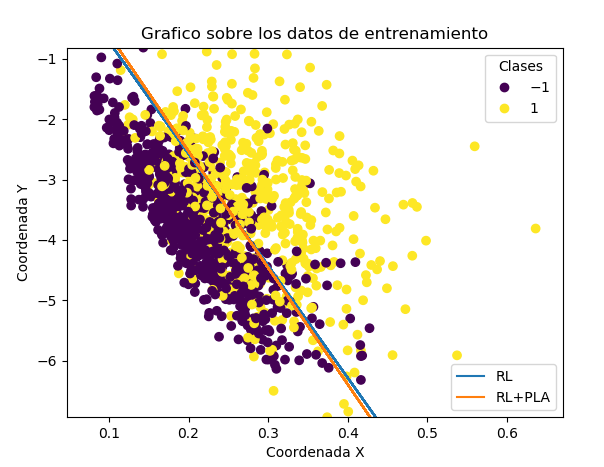
\includegraphics[width=0.7\textwidth]{./img/datos}
\caption{Conjunto de datos de entrenamiento junto con las funciones RL y RL+PLA.}
\end{figure}

\begin{figure}[H]
\centering
\spanishdecimal{.}
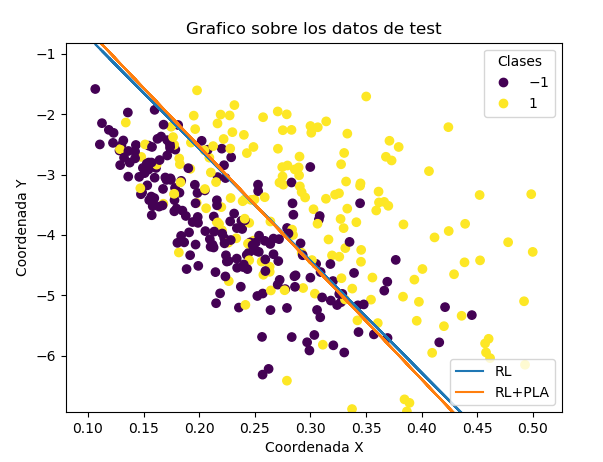
\includegraphics[width=0.7\textwidth]{./img/datostest}
\caption{Conjunto de datos de test junto con las funciones RL y RL+PLA.}
\end{figure}
\item Calcular $E_{in}$ y $E_{test}$ (error sobre los datos de test).

Utilizamos el conjunto de test dado para calcular el error de $E_{test}$.
\begin{verbatim}
Bondad del resultado para RL:

Ein:  0.22780569514237858
Etest:  0.2513661202185792
\end{verbatim}

\begin{verbatim}
Bondad del resultado para RL + PLA:

Ein:  0.22529313232830817
Etest:  0.25409836065573765
\end{verbatim}
Obsevamos que apenas hay mejoría, aunque los resultados ya antes de aplicarle el PLA eran bastante buenos, por lo que no nos resulta raro que no haya mucha mejora.

\item Obtener cotas sobre el verdadero valor de $E_{out}$ . Pueden calcularse dos cotas una
basada en $E_{in}$ y otra basada en $E_{test}$ . Usar una tolerancia $\delta = 0.05$. ?`Que cota es mejor?

Por la desigualdad de Hoeffding sabemos que, con probabilidad $1 - \delta$: 
$$E_{out}(g) \leq E_{in}(g) + \sqrt{\frac{1}{2N_{in}} \cdot ln \frac{2M_{in}}{\delta}} $$
$$E_{out}(g) \leq E_{test}(g) + \sqrt{\frac{1}{2N_{test}} \cdot ln \frac{2M_{test}}{\delta}} $$

Donde $N$ es el número de puntos en cada caso y $M$ es el cardinal del conjunto $H$. En el caso de $E_{in}$, $M_{in}$ sería infinito, por lo que introducimos el máximo de precisión en \textit{bits} necesarios para representar tres flotantes ($2^{64\cdot3}$). Por otro lado el valor de $M_{test}$ es $1$, porque ya hemos estimado la recta previamente y hemos elegido una concreta.

Veamos los resultados:
\begin{verbatim}
Cota superior de Eout con Ein:  0.46461547451143265
Cota superior de Eout con Etest:  0.32508746408835315
\end{verbatim}
Vemos que la mejor cota es $E_{test}$ porque es más pequeña que la de $E_{in}$.
\end{enumerate}
\end{enumerate}

%printbibliography

\end{document}
